The chromatin packaging of the genome plays a fundamental role in the gene regulation of eukaryotic individuals.
To study this aspect of the \gls{dna} several technologies have been developed, such as \textit{FAIRE-seq} \cite{Giresi2007}, \textit{DNase-seq} \cite{Winter2013}, \textit{ATAC-seq} \cite{Buenrostro2013}, etc.

\textit{ATAC-seq} among the others is having a growing interest and diffusion in the last years, because it offers comparable results to the \textit{DNASE-seq} with less biological material and less library preparation time.

\begin{figure}[h]
\centering
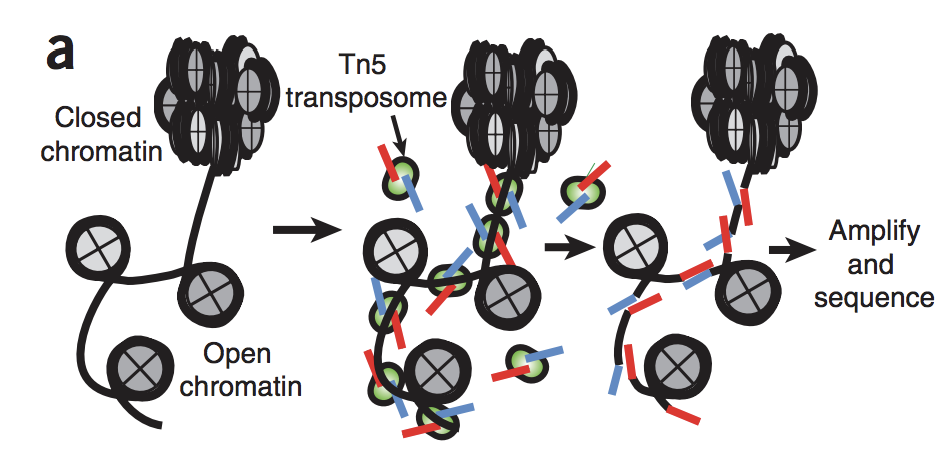
\includegraphics[width=9cm,keepaspectratio]{img/intro/atac.png}
\caption[ATAC-seq experiment]{Representation of \textit{ATAC-seq }library preparation. \cite{Buenrostro2013}}
\label{fig:atacseqexp}
\end{figure}

The library preparation adopts a hyperactive \textit{Tn5} transposase, modified with adaptors for high-throughput  \gls{dna} sequencing, which is able to fragment and tag a genome simultaneously.
The technology exploits the \textit{Tn5} capability of integrating itself into active regulatory elements.

After \textit{Tn5} tagmentation, the resulting segments can be amplified and sequenced, producing sequences to map on a reference genome.
There is no standard analysis reached for the \textit{ATAC-seq} analysis, but, inspired by the \textit{ChIP-seq} analysis, the resulting reads, typically, are processed with tools (peak callers) for quantifying their amplification, which produces for each detected open chromatin region a feature, the peak (generally with an associated score). 

Depending on the used tool, the peaks can be represented in different data structures, but their representation is typically given by the genomic coordinates; chromosome, starting and ending point of the region, the strand of the \gls{dna} on which the region lies, and additional attributes such as a score, a number of samples on which the regions have been detected, etc.

To obtain the first level of integration, the peaks can be annotated with other relevant features of the genome, such as the \gls{tss} of the genes, \gls{utr}, promoters, exons, introns, etc.  
Then, the annotated genes can be used to enrich for GO terms or pathways, reaching the second level of integration \cite{righelli2018, Koberstein2018, Ou2018}.




